\section{Architecture}
\label{sec:architecture}
This section will give an overview of the general concepts and will show with examples how to use the application.

\subsection{General concepts}
The complete code was structured with too general ideas in mind. On the one hand it should be modular in the sense that the application consists of components that can be reused on multiple occasions. For example a dialog for the deletion can be always the same and only the handling and the description text have to be adapted based on the usage. The modularity will be introduced implicitly by React, because the general idea is the creation of components that will be updated internally by react.

Another relevant aspect was the future extension of the application, in order to be able to integrate more steps for the creation of the configuration. For example adding additional properties for the subcomponent configuration.

\subsection{App-Component}
The App is the central component that will contain all the relevant components for the application. The App keeps track of the current configuration and provides the access for the components via a context provider. This allows the access and update of the configuration from all the components, which will also trigger the React lifecycle to re-render a component.

\subsection{Welcome page}
The welcome page is the first component that will be displayed when you start the application.
In figure \ref{fig:app_welcome} you can see that there are two buttons that allow to start the configuration. There are two choices on how to start the configuration, the start with an import and without an import, based on the choice a user makes the wizard (compare section \ref{sec:wizard}) will be started with different steps.

\begin{figure}[ht]
    \centering
    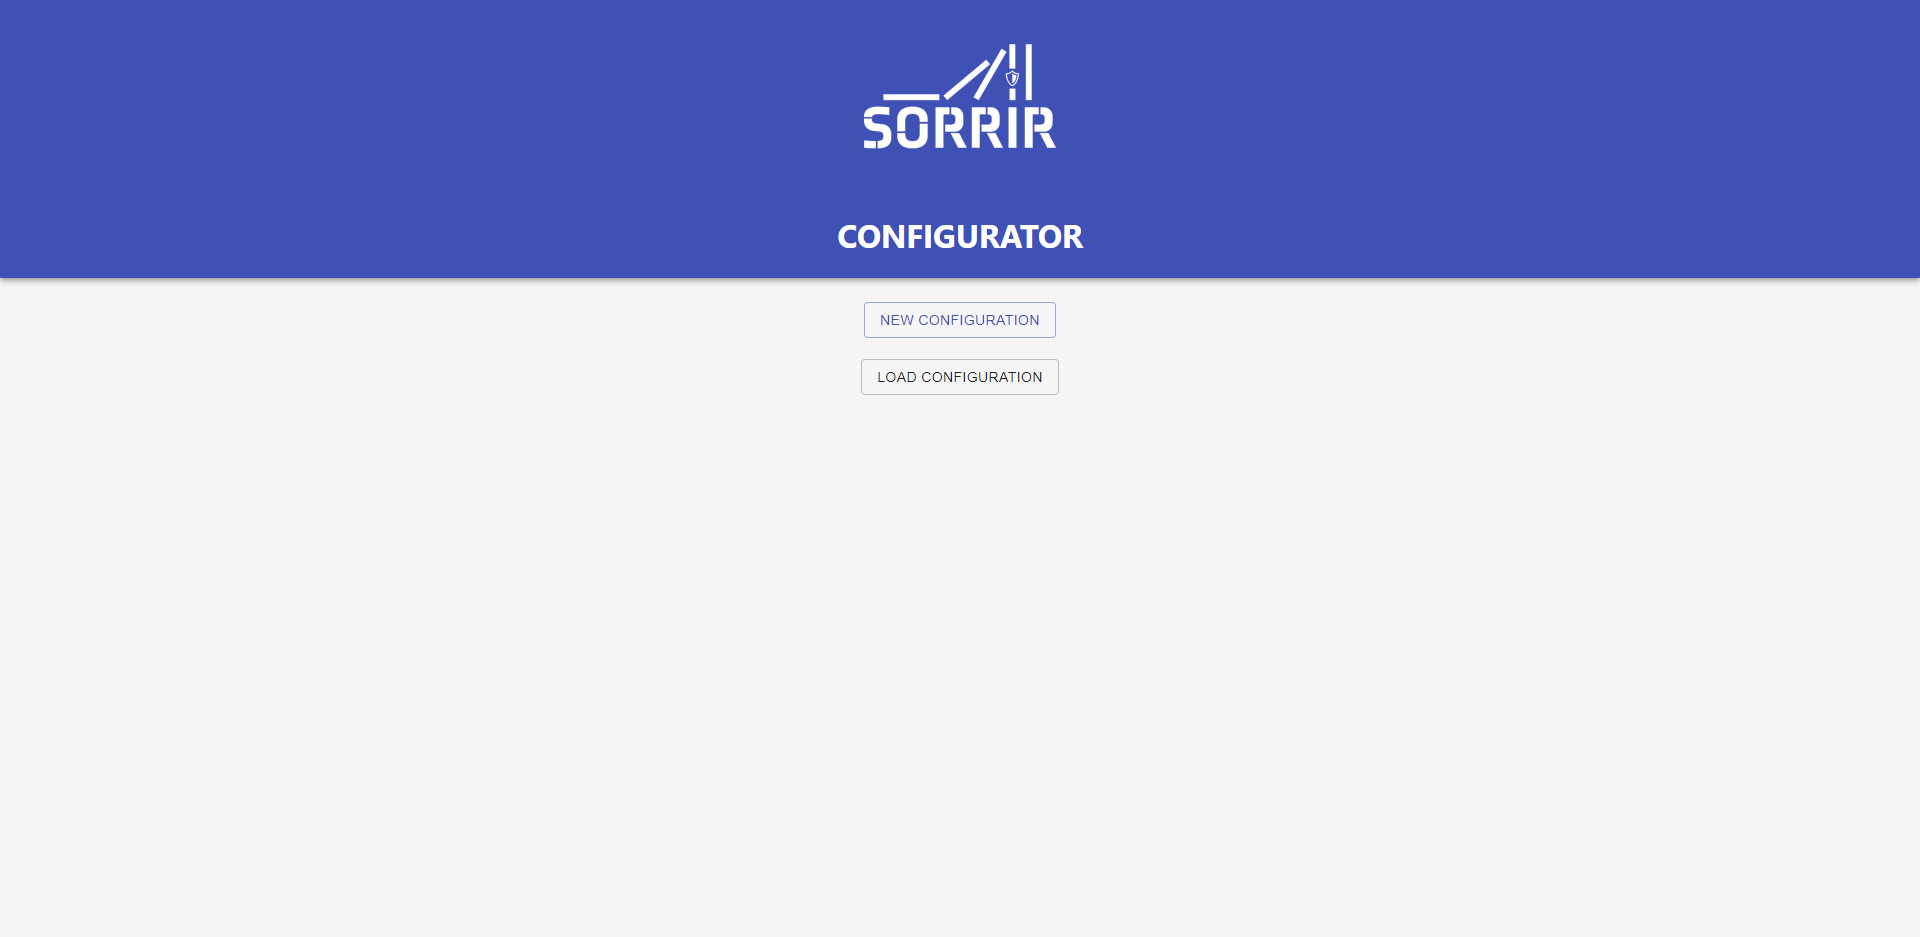
\includegraphics[width=\textwidth]{img/app_welcome.png}
    \caption{Welcome page}
    \label{fig:app_welcome}
\end{figure}

\subsection{Wizard}
\label{sec:wizard}
The creation of the configuration can be divided into several steps. To facilitate the configuration, a wizard has been developed that allows the step-by-step configuration. In addition to that it is also possible to navigate arbitrary back and forth between the different steps of the configuration. 

The wizard component allows to dynamically configure what steps will be shown and in what order. The wizard consist in general of a menu-bar, a stepper to show navigate between the steps and the content it will show which is internally called a view. 

Figure \ref{fig:wizard} shows the menu bar and the stepper for the configuration with an import. You can navigate through the different steps by clicking on the steps in the stepper, whereby the active step is highlighted. The menu bar will update its label with the label that was specified for the current step, for example in the figure the label was set to "Import".

\begin{figure}[ht]
    \centering
    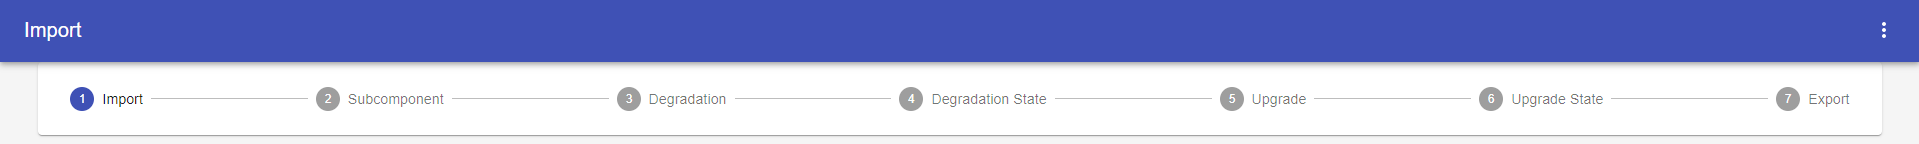
\includegraphics[width=\textwidth]{img/wizard.png}
    \caption{Wizard}
    \label{fig:wizard}
\end{figure}

\noindent In addition to the navigation between the different steps there is a menu on the top right. At the moment this only has one menu item that allows to restart the configuration, but it is possible to further add more functionality. The restart will show a dialog to confirm the reset of the current configuration and will, after the confirmation, send the user back to the welcome page. \\

\noindent In order to extend the wizard with additional steps following actions have to take place:

\begin{itemize}
    \item Extension of the view enum ( a enum that contains all available views in the application) ("src\textbackslash util\textbackslash Views.ts")
    \item Setting a label for the new view ("src\textbackslash util\textbackslash ViewLabelResolver.ts")
    \item Adding the view that will be displayed for the step in the wizard. This has to be a react component ("src\textbackslash components\textbackslash wizard\textbackslash ViewSelector\textbackslash ViewSelector.tsx")
\end{itemize}

\noindent After these steps the wizard can be configured to display the new view as an additional step.

\subsection{Import}
The import view is only inserted as a step when the wizard is started with the "LOAD CONFIGURATION" button on the welcome page. The import page allows to import an existing configuration file and will update the current configuration in the app. This import will also override all previous changes in the configuration. The configuration will be displayed with syntax highlighter that will be updated with the new configuration after the import was successful. 

There are several cases when the import has to fail to enforce a correct state of the configuration and therefore it will be validated that file contains a valid configuration. If this is not the case the import will display any errors that occurred during the import. The first part of the validation is to check if the file contains an object that can be parsed to a json object. if this is not the case an error message similar to the message in figure \ref{fig:import_invalid_file} will be displayed.

\begin{figure}[ht]
    \centering
    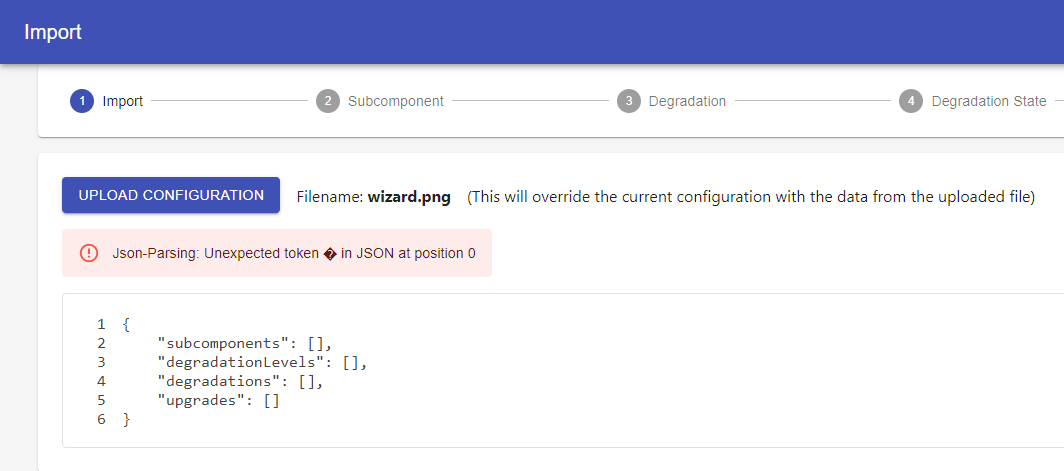
\includegraphics[width=\textwidth]{img/import_invalid_file.png}
    \caption{Import invalid file}
    \label{fig:import_invalid_file}
\end{figure}

\noindent The second part of the validation is the validation of the json object itself. The json object requires several properties to be a valid configuration. Details on this part of the validation can be found in section \ref{sec:validation}.
The validation may also find several problems for the imported file that will be displayed as shown in figure \ref{fig:import_invalid_json}. If the problem occurs in an element of an array, for example in the subcomponents, the index of the element will also be added to the error message.

\begin{figure}[ht]
    \centering
    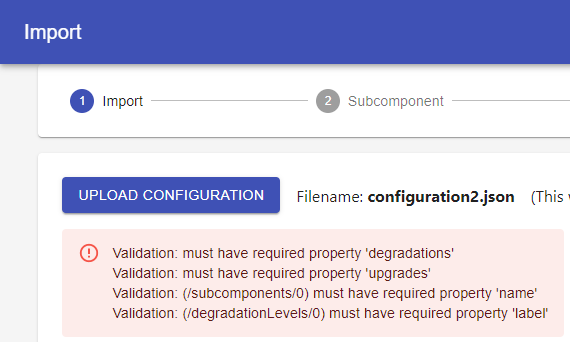
\includegraphics[width=0.8\textwidth]{img/import_invalid_json.png}
    \caption{Import invalid json}
    \label{fig:import_invalid_json}
\end{figure}

\subsection{Validation}
\label{sec:validation}
\begin{itemize}
    \item Validates if the file can be parsed as Json element
    \item If it can be parsed the validation will be done
    \item short explanation of the different schema types?
    \item use of ajv ( support of JSON Schema and JSON Type Definition)
    \item atm most tools support Json Schema (cite \url{https://ajv.js.org/guide/schema-language.html})  $\rightarrow$ selection for our usecase - but no offical RFC only internet draft
    \item ajv used because it supports both - migration later possible (to RFC8927 JSON Type Definition)
    \item Short overview of the implemented schema for the configuration (perhaps using UML diagram)
\end{itemize}

\subsection{Subcomponent configuration}
\begin{itemize}
    \item Subcomponents required for the creation of degradation levels
    \item Subcomponent has an id, a name and several shadowmodes (internal state of the subcomponent)
    \item each shadowmode has an id and a name 
    \item In order to be able to manage the relevant subcomponents for the component, a table with a creation/edit and deletion dialog is offered
    \item The creation/edit dialog offers several functions: 
        \begin{itemize}
            \item Internal validation function (non empty fields + check for already existing subcomponents with the same id)
            \item id autofill ( based on the name) if no value is set
        \end{itemize}
\end{itemize}

\subsection{Degradation Level Management}
\begin{itemize}
    \item Creation/Deletion in the Degradation and Upgrade Configuration views
    \item Create/Edit with a Dialog:
    \begin{itemize}
        \item name and id as string
        \item the subcomponent states of the level (will show all possible values of a subcomponent and to choose what has to be true for this level)
        \item creation of internal states of the Level (with custom chip input)
        \item validation if id exists/ etc.
    \end{itemize}
    \item Multi selection in the Degradation and Upgrade Configuration View
\end{itemize}

\subsection{Degradation and Upgrade configuration}
\begin{itemize}
    \item Custom Graph View for the Hierarchy (Recursive generation of the Graph)
    \item Drag and Drop Support to update the Graph (degradation level hierarchy)
    \item Off state as default node
    \item Explain model on how to save the hierarchy (LevelChange model) 
    \item shows all levels even the ones that are not inserted in the hierarchy yet
    \item Upgrade: Inverse of the Degradation Graph - same functionality as Degradation Graph
    \item Both will be saved separately in the configuration and are also separate steps in the wizard
\end{itemize}

\subsection{LevelChange configuration}
\begin{itemize}
    \item configure the state in which the level after the degradation or upgrade is
    \item separate step in the wizard for both degradation and uprade
    \item shows for all LevelChanges the states of the corresponding level and allows the selection of the state the level will be in after the degradation/upgrade 
\end{itemize}


\open{Use figures for the different sections (e.g. import successful and unsuccessful)}